\documentclass[journal]{IEEEtran}
\IEEEoverridecommandlockouts
% The preceding line is only needed to identify funding in the first footnote. If that is unneeded, please comment it out.
\usepackage{amsmath,amssymb,amsfonts}
\usepackage{graphicx}
\usepackage{textcomp}
\usepackage{xcolor}
\usepackage{listings}
\usepackage{natbib}
\usepackage{hyperref}
\usepackage{enumitem}
\colorlet{punct}{red!60!black}
\definecolor{background}{HTML}{EEEEEE}
\definecolor{delim}{RGB}{20,105,176}
\colorlet{numb}{magenta!60!black}

% correct bad hyphenation here
\hyphenation{op-tical net-works semi-conduc-tor}

\begin{document}
\def\HS{\hspace{\fontdimen2\font}}\the\fontdimen2\font
\title{Delegated Anonymous Credentials with Revocation Capability for IoT Service Chains}
\author{\IEEEauthorblockN{\textsf{Sandeep Kiran Pinjala}$^{1,2}$ and
    \textsf{Krishna     M. Sivalingam}$^1$}

\IEEEauthorblockA{\textit{$^1$Dept. of Computer Science and
    Engineering, Indian Institute of Technology Madras, Chennai, India} \\ 
\textit{$^2$HCL Technologies, Chennai, India} \\
\texttt{\footnotesize{Email: sandeepkiranp@gmail.com, cs16s001@smail.iitm.ac.in,
skrishnam@iitm.ac.in, krishna.sivalingam@gmail.com}}
}}

\IEEEoverridecommandlockouts
\IEEEpubid{\makebox[\columnwidth]{978-1-5386-4980-0/19/\$31.00
    \copyright2019 IEEE} \hspace{\columnsep}\makebox[\columnwidth]{ }}

\maketitle

\begin{abstract}
The abstract goes here.
\end{abstract}

% Note that keywords are not normally used for peerreview papers.
\begin{IEEEkeywords}

\end{IEEEkeywords}



\IEEEpeerreviewmaketitle



\section{Introduction} \label{introduction}

Internet of Things (IoT) enables physical objects also called \textit{Things}  to communicate with each other and to their human operators over the internet. This opens up a myriad of use cases such as smart homes, smart factories, smart cities, smart healthcare, smart grids etc \cite{IoT}. It is also expected that such connected devices could reach upto 50 billion by 2020 \cite{Evans}. The IoT devices (for example, a smart bulb or a temperature sensor) are very constrained in terms of memory, processing power, storage and most often are battery powered. Unlike the traditional computers these devices cannot perform computationally intensive tasks and are intended for minor operations of sensing and actuation. Most of these devices are out in the open without any physical supervision making them easily susceptible to physical attacks.

Owing to the resource constraints and physical openness, IoT devices have been targets of various attacks \cite{iot-sec} at physical, network and application layers. IoT devices also collect lot of personal information like user's location, eating habits, medical history etc of its users because of which there has been a growing concern among consumers of such services. Unlike normal computers, these devices cannot provide an interface where the user can look up what personal information is being shared and with whom. In \cite{Ziegeldorf2014PrivacyIT} the authors define privacy in IoT as a guarantee for the subject	

\begin{enumerate}[label=\alph*)]
	\item To be aware of the privacy risks imposed by smart things.
	\item Control over collection and processing of personal information
	\item Control over subject's personal information being disseminated outside of his control sphere.
\end{enumerate}
They then categorize privacy threats and challenges of IoT into a) Identification b) Localization and tracking c) Profiling d) Privacy-violating interaction and presentation e) Inventory and life cycle tracking and f) linkage.

IoT services do not act in silos. They interact with each other and with external entities to provide a complete package of services to the user. For example, in Home Automation, based on the user who is entering the house (say Owner vs Guest), a completely different set of services may get invoked. The service interactions and invocations depend on the roles and capabilities of the user invoking them. We call the sequence of services that get invoked as \textit{IoT Service Chain}. In this paper we look at providing security and privacy to users and IoT devices that invoke IoT service chains. The rest of the paper is organized as follows. Section \ref{motivation} describes the motivation, problem statement and our contribution. Section. \ref{preliminaries} talks about the preliminaries on which the system is built. Section \ref{camen} talks about the anonymous credential mechanism that we will use in our scheme. Section \ref{proposal} talks about the architecture and the components. In Section \ref{seceval} we evaluate the security aspect of the proposal and in Section \ref{implementation} we talk about the implementation aspects and the results.

\section{Motivation and related work} \label{motivation}

\subsubsection{IoT Service Chains} \label{iotsvcch}
We introduced \textit{IoT Service Chains} in Section \ref{introduction} to refer to the chain of services invoked when an event occurs. Individual services in the chain interact with each other, on-behalf of the initiator towards a common goal. Initiator could either be a human or an IoT device. Each service in the chain would in-turn validate the user/IoT device's credentials for the desired service functionality. IoT devices can either act on behalf of their operator or can be independent of it. For example, if a smart Heart Monitoring System (HMS) detects a low pulse rate for a patient, it immediately needs to initiate the Advanced Cardiac Life Support (ACLS) by injecting an IV of an antidote, reading and interpreting the ECG, starting CPR, inform the doctor etc. The HMS in this case acts as an independent device and does not impersonate the patient. But in case of a smart fridge, which keeps track of the stock of milk, it automatically places an order for replenishment by using the owners credit card details. In this case, the smart fridge acts on behalf of the owner.

\begin{figure}[htbp]
\centerline{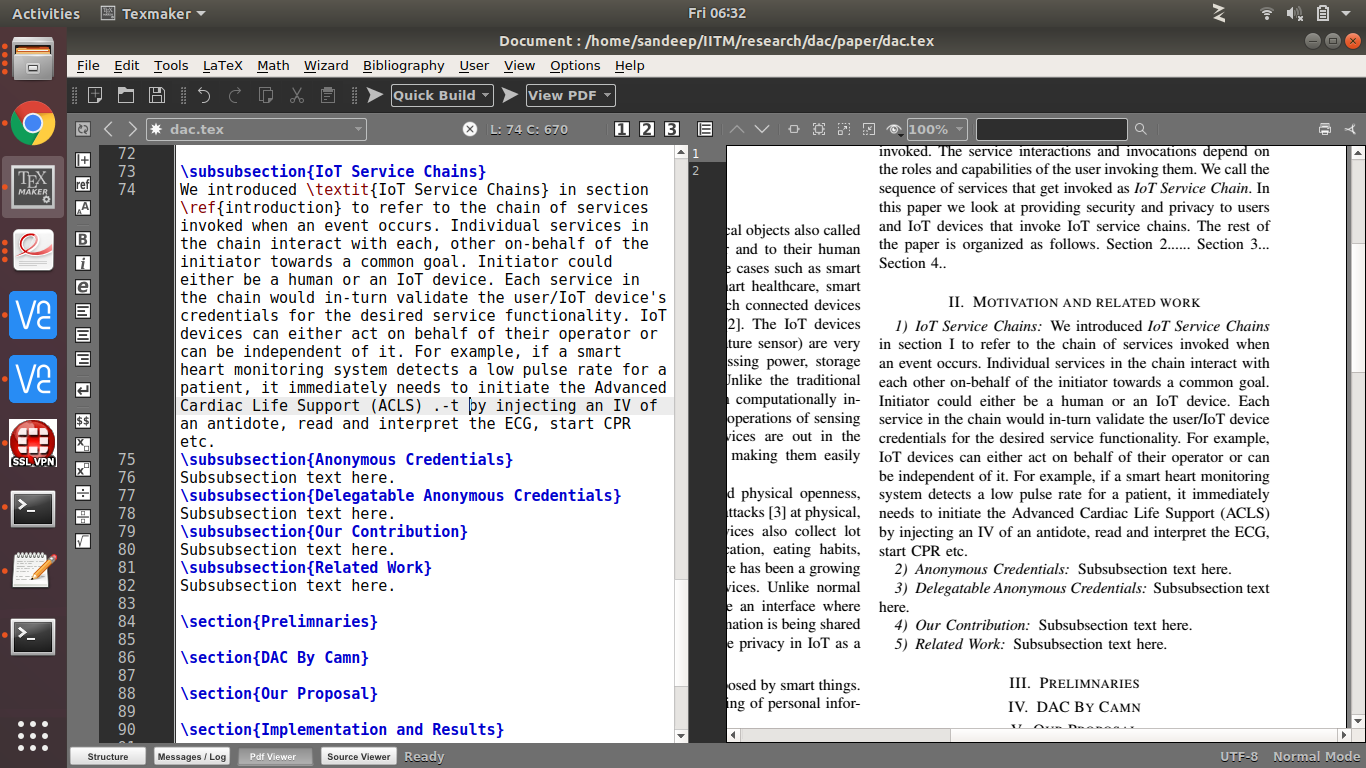
\includegraphics[width=3in]{dac.png}}
\caption{IoT Service Chain}
\label{fig:iotsvc}
\end{figure}

As can be seen in Fig.~\ref{fig:iotsvc} there are 5 services in the IoT service chain. xxxx explanation of HMS, ACLS etc interactions among services, authentication etc

One thing to notice from the above figure is that while the service chain is being invoked, the user/IoT device has to be online so that it supplies the necessary credentials for authentication and authorization.  This isn't a huge problem if the initiating entity is a user (having a smart phone or a tablet). But for a constrained IoT device generating authentication and authorization information for each service in the chain would quickly result in draining of its resources. Also, most of the IoT devices are duty cycled and may not remain active till the chain completes. This again results in loss of packets or in retransmission. It will be even more challenging if the user/device's privacy needs to be protected through out the chain. In this paper we focus on some of the options on how user or device privacy can be ensured when invoking the service chain without pushing the device to its resource limits.

\subsubsection{Attribute Based Anonymous Credentials}
In traditional credential based system, a central authority grants credentials to users and systems. These credentials can be password or token (for example, certificate) based. When the user wants to access a resource he presents the credential to it which inturn validates the credential. The resource (also called service) trusts the central authority and thereby the credentials issued by it. Once the credential verification is done, the service checks whether the user has got the right access level to access the resource. One of the primary concerns with such a system is that the service gets to know the complete details of the user presenting the credential. For example, when user's Digital Certificates are presented for access, the service will know how long the credential (certificate in this case) is valid, the country, state, organization, email address etc of the user, who are all the intermediate chain of issuers etc. The only information that matters to the service is whether the certificate is valid and is issued by the central authority and whether the user possesses the required access rights. But in this case lot more user details are available to it. With so much personal information available to the service, there is always a chance of misuse of data if it falls in wrong hands. According to European Union General Data Protection Regulation (GDPR) Data Minimization principle, entities should only process adequate, relevant and limited personal data that is necessary in relation to the purposes for which they are processed. As mentioned in \cite{Ziegeldorf2014PrivacyIT}, the privacy problem becomes manifold in IoT world. One, because there are huge number of constrained IoT devices without proper security measures in place. And two, there is very little control over what personal information is disseminated from these devices to the outside world.

Anonymous Credentials introduced in \cite{chaum83blindsign} provide a way in which a user can prove that he holds a credential without revealing any information about the user. The verifier cannot also forge the user's credential. In Attribute Based Anonymous Credentials, a user can selectively prove that he holds the set of attributes needed by the verifier and not reveal all of his attributes, thereby maintaining privacy. The user creates a zero-knowledge proof of possession of the credential which the verifier verifies using the public key of the central authority. Some of the most popular Anonymous Credential Systems (ACS) are \cite{CamenischH02} and \citep{uprove}.

A Delegatable Anonymous Credential (DAC) System, introduced in \cite{delegatabledac} not only allows the users to generate anonymous credentials, but also allows them to anonymously delegate their credentials to other entities. For example, in a hierarchical setup, the root issuer may delegate its issuing authority to region wise issuers who in turn may delegate to division wise issuers and so on. Although there can be multiple levels of delegation, the anonymous credential generated by the prover at any level can only be verified by the public key of the root issuer.  One of the primary advantages of DAC is that it alleviates the burden on the root issuer to issue credentials but still maintains anonymity of all the issuers in the chain.

\subsubsection{Our Contribution}
In section \ref{iotsvcch} we talked about IoT service chains and the difficulty of ensuring user/IoT device's privacy during the chain propagation. We address this problem with our proposal on \textbf{\textit{Delegated Anonymous Credentials in IoT Service Chains}}. We describe a mechanism in which the IoT device can delegate its credentials to a Controller which in turn generates an anonymous credential based on the attributes needed by the service. Our scheme is based on the DAC system developed by Camenisch \textit{et al.} \cite{CamenischDD17}. The authors developed a scheme where credentials are not delegated anonymously but the presenter anonymously proves that the entire chain of delegation is valid. The verifier verifies the anonymous credential just with the root issuer's public key.

The following are major contributions in this work.
\begin{enumerate}[label=\alph*)]
	\item Discuss in detail the problem of ensuring privacy to users and IoT devices in IoT service chains.
	\item Implementation of the DAC scheme outlined in \cite{CamenischDD17}. We used the Pairing Based Cryptography Library from \cite{pbc} for the implementation. We implemented the full L-level credential Delegation, Presentation and Verification.
	\item Credential revocation has been mentioned as "future work" in \cite{CamenischDD17}. We extended \cite{CamenischDD17} to incorporate credential revocation.
	\item Once the verification of the anonymous credential token completes, the next logical step would be to communicate with the prover to exchange data. In order to do that securely, a common session key needs to be established between the two parties. We demonstrate how the session key can be established.
	\item We then used the above DAC implementation to realize Delegated Anonymous Credentials in IoT service chains. We outline the framework consisting of Root issuer, Controller, User/IoT device and Service as the principal components. We describe the messages exchanged between these components and outline how privacy of users can be ensured.
	\item We implemented the above scheme and discuss the various possibilities on how token verification and policy implementation can happen for constrained IoT services. Various metrics like time taken, number and size of messages exchanged, memory, CPU etc are evaluated for the various models that we discuss. 
\end{enumerate}

\subsubsection{Related Work}
Subsubsection text here.

\section{Preliminaries} \label{preliminaries}
In this section we introduce some of the concepts related to DAC building blocks. 

\subsubsection{Bilinear map}
A Bilinear map is a Pairing-Based Cryptography construct that allows us to build and analyse cryptographic systems. Let $G_1$, $G_2$ and $G_T$ be multiplicative groups of order $q$, then a bilinear map $e : G_1 X G_2\rightarrow G_T$ satisfies the following properties

\textbf{Bilinearity}

$$\forall P \in G_1, \forall Q \in G_2 : e(P^a, Q^b) = e(P,Q)^{ab}$$

\textbf{Non-Degeneracy}
$$ A \neq 0 \Rightarrow e(A,A) \neq 1$$

\textbf{Computability}

\HS\HS\HS\HS \HS\HS e is efficiently computable


\subsubsection{Zero Knowledge Proofs}
Zero knowledge Proofs (ZKP), introduced in \cite{zkp} allow the prover to prove that he knows certain information without revealing the information (or anything related to it) to the verifier. A ZKP should be complete, sound and should not reveal any information from the proof. A zero-knowledge proof of knowledge is a special case where the prover possesses a secret information and not just the knowledge of it. Interactive ZKP require interaction between the prover and the verifier to prove that the prover has the secret information. For example, the Schnorr ZKP is outlined in \cite{rfc8235}. The Non-Interactive ZKP (NIZKP) proofs do not require any kind of interaction for the proof to proceed. The Schnorr NIZKP proof is obtained through the Fiat-Shamir transformation \cite{Fiat1986HowTP}.

\subsubsection{Signature Schemes}
A signature scheme consists of the following algorithms.
\begin{enumerate}[label=\alph*)]
	\item Setup : Given the security parameter, the algorithm outputs public parameters.
	\item Key Generation : This algorithm generates a public key and the corresponding private key based on the public parameters.
	\item Signature Generation : This algorithm takes the private key and the message and outputs the signature. The generated signature should not be forge-able.
	\item Signature Verification : This algorithm takes the signature, public key and the message and outputs whether the verification is successful or not.
	
\cite{CamenischDD17} uses Groth's structure preserving signature scheme \cite{groth} where the public keys, messages to be signed and the signatures are all elements of group $G1$ or $G2$.

\end{enumerate}

\section{DAC By Camenisch \textit{et al.} \cite{CamenischDD17} and our extensions} \label{camen}
The authors in \cite{CamenischDD17} built a practical attribute based DAC system of L-level hierarchy where the delegation is not anonymous. The delegator reveals its identity and the identity of the entire chain to the delegatee during the delegation process. It is only during the presentation of the anonymous credential, the prover hides the identity of all the intermediate delegators. The prover also selectively reveals attributes at each level of delegation. The verifier in turn uses the root issuer's public key to verify the anonymous credential token. The authors also describe the instantiation of their DAC system based on Groth \cite{groth} and Schnorr \cite{rfc8235} schemes. The authors introduce a new signature scheme called \textit{sibling signatures} which allows a users with a single key pair with two different signature schemes. This single key pair can be used both during delegation and token presentation.

\begin{figure}[htbp]
\centerline{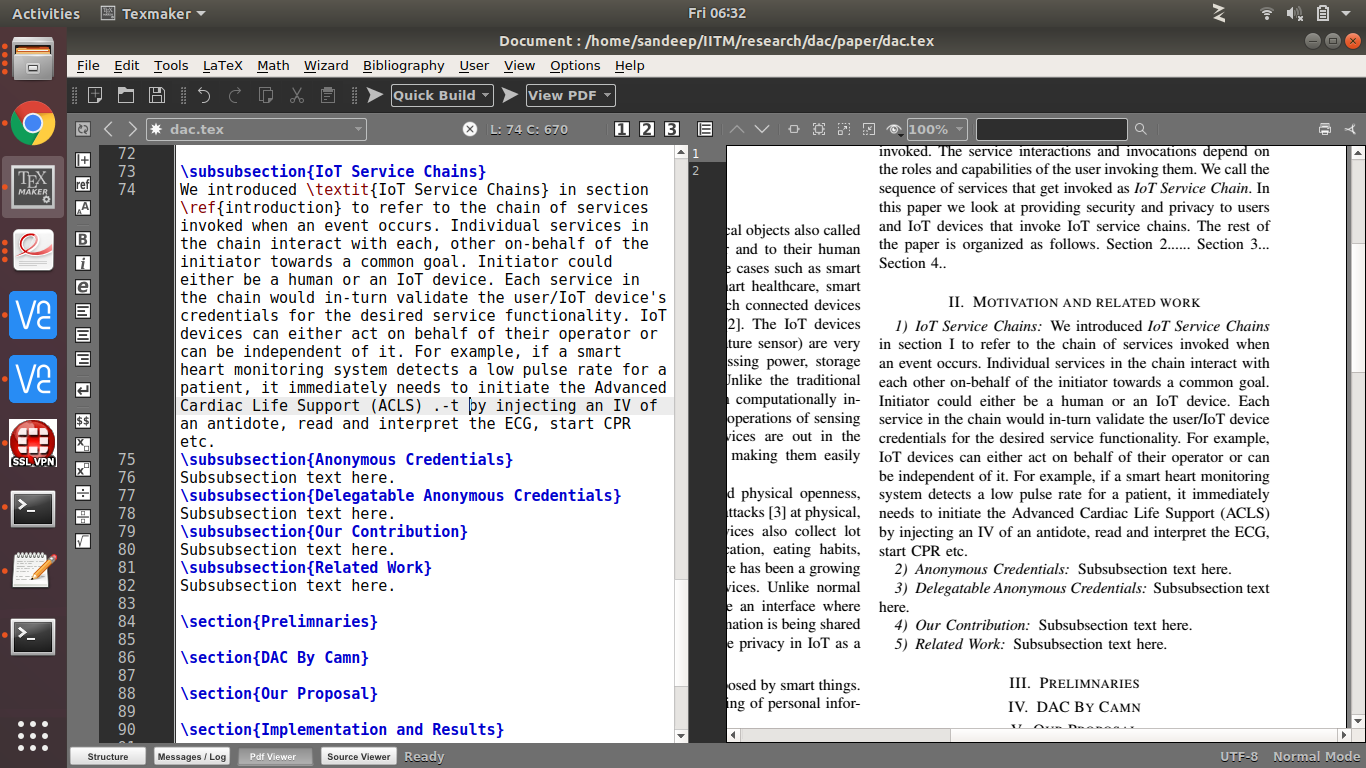
\includegraphics[width=3in]{dac.png}}
\caption{Generic Construction of Camenisch \textit{et al.} \cite{CamenischDD17}}
\label{fig:genconst}
\end{figure}

The author's generic construction scheme is depicted in Fig. \ref{fig:genconst}. At Level-0 is the root issuer with public, private key pair as $(ipk,isk)$. The root issuer delegates certain attributes $\overrightarrow{a_1}$ to $user1$ at Level-1 with key pair as $(cpk_1, csk_1)$. It generates a signature $\sigma_1$ on the combination of $(cpk_1,\overrightarrow{a_1})$ using $isk$. It passes on the signature and attributes to  $user1$. Similarly, if $user1$ at Level-1 wants to delegate certain attributes $\overrightarrow{a_2}$ to $user2$ with key pair $(cpk_2, csk_2)$, it generates a signature $\sigma_2$ using $csk1$ over $(cpk_2,\overrightarrow{a_2})$. $user2$ then forwards the $\sigma_1$, $\overrightarrow{a_1}$ and $cpk_1$ generated at Level-1 as well as $\sigma_2$, $\overrightarrow{a_2}$ generated at Level-2 to $user2$. This can go on till any Level-$l$ credential. So a Level-$l$ credential is a combination of all signatures, attributes and public keys of all $l-1$ levels and Level-$l$ private key.

In order to anonymously present a credential at any level, the prover generates a NIZKP proof proving that he holds the entire credential chain (signatures, attributes and public keys at each level). He can selectively reveal attributes at each level. The public keys (and thereby the identity of users) at each level will remain hidden. The verifier verifies the token using just the root issuers public key $ipk$. The authors provided an instantiation of their construction scheme using Bilinear Pairings and Groth-Schnorr sibling signatures. They used Groth1 to denote Groth signatures on messages in $G1$ with public key in $G2$ (called SibGS1) and Groth2 to denote Groth signatures on messages in $G2$ with public key in $G1$ (called SibGS2). The final attribute token would then look like

\begin{multline}
$$
at \leftarrow NIZK \lbrace(\sigma_1,...,\sigma_L,cpk_1,...,cpk_L,<a_{i,j}>_{i \notin D},tag) : \\ 
\bigwedge \limits _{i=1,3,..} 1 = SibGS1.Verify_1(cpk_{i-1}, \sigma_i,cpk_i,a_{i,1},...a_{i,n_i})\\
\bigwedge \limits _{1=2,4,..} 1 = SibGS1.Verify_1(cpk_{i-1}, \sigma_i,cpk_i,a_{i,1},...a_{i,n_i})\\
\wedge 1 = SibGSb.Verify2(cpk_L,tag,m)\rbrace
$$
\end{multline}

In order to prove that the prover holds the private key corresponding to the public key at Level-L($cpk_L$), the NIZK proof also includes the proof for a message $m$ signed with the private key at Level-L ($csk_L$). In the concrete instantiation, this proof of private key possession is later turned into Schnorr signature proof of knowledge using Fiat-Shamir heuristic.

\subsubsection{Credential Revocation} \label{revoke}
One of the important functionalities of any credential based system is to account for revoked credentials. Revocation allows the administrator to stop rouge elements from entering into the system. The authors in \citep{CamenischDD17} left out credential revocation as a future item. In this section we discuss how credential revocation can be achieved using the author's concrete instantiation.

As mentioned in the previous section, if a user at level K-1 wants to delegate certain attributes ($\overrightarrow{a_K}$) to another user, he signs the message $(cpk_K,\overrightarrow{a_K})$ with $csk_{K-1}$. We propose to extend the signature message to include a Hash of $(cpk_K , \overrightarrow{a_K})$. We call this hash as the credential hash at level K. Therefore,

$$
h_K = Hash(cpk_K,\overrightarrow{a_K})
$$
$$
\sigma_K = Sign_{csk_{K-1}}(cpk_K,h_K,\overrightarrow{a_K})
$$

Hash in this case can be one of the \textit{Secure Hash Algorithms} in the SHA-2 family. The credential hash is a unique representation of the public key and the delegated attributes at any level. Since the signature includes the credential hash, signature verification would fail if the hash is tampered. The delegator forwards $\sigma_K, h_K, \overrightarrow{a_K}$ to the delegatee. $h_K$ forms a part of credential at every level. The attribute token generated for presentation would now look like

\begin{multline}
$$
at \leftarrow NIZK \lbrace(\sigma_1,...,\sigma_L,cpk_1,...,cpk_L,<a_{i,j}>_{i \notin D},tag) : \\ 
\bigwedge \limits _{i=1,3,..} 1 = SibGS1.Verify_1(cpk_{i-1}, \boldsymbol{h_i}, \sigma_i,cpk_i,a_{i,1},...a_{i,n_i})\\
\bigwedge \limits _{1=2,4,..} 1 = SibGS1.Verify_1(cpk_{i-1}, \boldsymbol{h_i},\sigma_i,cpk_i,a_{i,1},...a_{i,n_i})\\
\wedge 1 = SibGSb.Verify2(cpk_L,tag,m)\rbrace
$$
\end{multline}

When generating the attribute token, unlike other attributes, the credential hash value is always revealed to the verifier. There is no danger of someone modifying the hash as that would result in signature verification failure. If the root issuer or any delegator in the chain needs to revoke a credential, he would publish the credential hash in a Black List (BL) of credential hashes. The verifier has to check the credential hash for each level against the BL and if there is a match,  verification should fail.

The instantiation of the NIZK for the attribute token would now look like,


xxxxxx 


xxxxxx

\subsubsection{Session Key Establishment}
In the IoT scenario, once the token generated by the IoT device/User is verified by the IoT service, the next logical step would be to exchange data. In order to securely perform data exchange, both the endpoints should establish a common secret key. In the earlier section, we talked about how the authors use signature proof of knowledge over message $m$ to prove the possession of the Level-L private key. The proof then acts as a Digital Signature over $m$. Instead of any random message, the prover can generate an ephemeral public, private key pair ($pk,sk$) and use the public key $pk$ as the message over which the signature proof is performed. This public key is also sent along with the attribute token to the verifier. Once the token verification succeeds, the verifier generates a random secret key and uses the prover's ephemeral public key to encrypt it. It then sends the encrypted secret key over to the prover which then decrypts it using the private key $sk$. Any attempt by a Man-In-The-Middle to modify the public key sent to the verifier would result in the token verification failure. The scheme assumes that the response from the verifier is not tampered. Additional measures will have to be taken if verifier's identity and its response have to be validated at the prover.

\section{The Proposal} \label{proposal}
In this section we discuss in detail the architectural components of our proposal and the messages exchanged between them. One of the primary requirements of the system was to provide a light weight solution for IoT devices and users to anonymously access IoT services. 

\begin{figure}[htbp]
\centerline{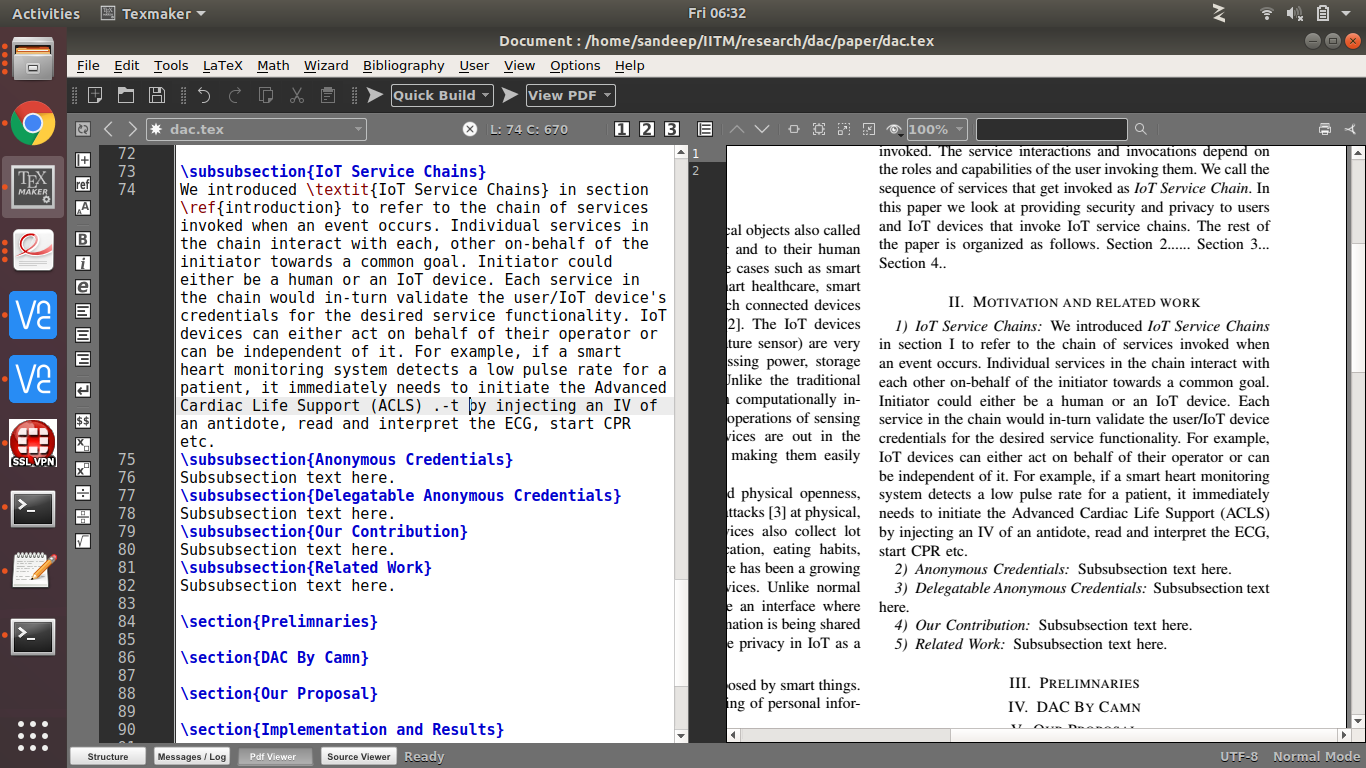
\includegraphics[width=3in]{dac.png}}
\caption{System Architecture}
\label{fig:sysarch}
\end{figure}

Fig. \ref{fig:sysarch} illustrates the system architecture with the following major components.

\subsubsection{The Root Issuer}
As the name implies, the Root Issuer (RI) issues Level-1 credentials to users/IoT devices. The RI service maintains a public, private key pair $(ipk,isk)$ using which it signs the Level-1 credentials. The public key $ipk$ is distributed across the system so that services can validate credential tokens presented from any delegation level just by using $ipk$.

The RI generates the system public parameters $G1, G2, g1, g2$ and the bilinear map $e$ when it is initialized for the very first time.

All users/IoT devices are assumed to hold one long term public, private key pair. Any user/IoT device which wishes to obtain credentials from RI, submits the credential request containing their public key and the attributes that they wish to possess. RI then validates the entity's request and generates the credential. As mentioned in section \ref{revoke}, RI signs the combination of user/device's public key, the credential hash and the attributes, with its private key $isk$. the credential hash is the hash of the user's publick key and all the attributes that the RI wishes to assign to the entity. The entity's credential would then be a combination of the signature, the credential hash, the attributes and its public, private key pair.

If the root issuer wishes to revoke an entity's credential, it would publish the credential hash in a BlackList (BL) that is available for everyone in the system to view. Only the RI can add, delete or modify the entries in the BL. Since the credential hash is hashed over public key and attributes, no one can infer any useful information about the entity just by looking at the hash.

\subsubsection{The Controller} \label{controller}
The Controller forms the core of the system. One of the primary reasons for choosing a centralized controller based approach is to allow the flexibility for both constrained devices as well as resourceful endpoints to anonymously authenticate and authorize against services. Even on the services end, constrained IoT services for example a smart bulb do not have the resources to validate an anonymous credential. With our approach, we allow both less constrained and very constrained endpoints to participate in the system. Some of the core functionalities of the Controller are

\begin{enumerate}[label=\alph*)]
	\item Accepts Delegated Credentials from Users/IoT devices and generates Anonymous Credentials to be presented to services in the IoT service chain.
	\item Maintains the list of system generated events and the corresponding services to be invoked.
	\item Maintains session information like services that were invoked, what attributes are needed for each service and so on for the entire service chain.
	\item Validates the User/Device credential against BlackListed credentials.
\end{enumerate}
On startup, the Controller loads the system parameters, generates public and private keys if this is the first time it is starting or loads the stored public and private keys. The Controller maintains a list of all the attributes required by each service in the system. This allows the Controller to generate anonymous credentials on behalf of the user/device by selectively revealing only the attributes required by the service and hiding the remaining ones. 

IoT devices/Users generate events when there is a change in normal behaviour. For example, the HMS detecting a low pulse rate for the patient, an intruder trying to enter the house, component breakdown in a shop floor etc. All these activities generate system events which are processed by the Controller. The Controller maintains a list of the services that need to be invoked for each event. For example, if a Guest enters the Smart Home, access to only the Guest room needs to be allowed, the Guest preferred lighting and temperature needs to be set and so on. Once an event is detected, the Controller invokes the corresponding services maintained in its list. Each service may in turn invoke other services in a chained manner. Each service in the chain validates if the user/device that generated the event has the required attributes to fulfil the service request. This continues till all the services in the chain are invoked. The controller also maintains a list of invoked services in the chain so as to avoid repeated invocations of the same service.

To elaborate more on the technical details, when a User/IoT device detects an event, it informs the Controller of the event. As part of the signalling mechanism, the IoT device delegates its credentials to the Controller. The device delegates all its attributes to the Controller. See section \ref{iotdevice}. On receiving the delegated credential and the event, the Controller first verifies the delegated credential using the Root Issuer's public key $ipk$. It also checks if the user's credentials are black listed or not. If the delegated credential is fine, it would then retrieve the list of services that need to be invoked for the event. For each such service, the Controller generates an anonymous credential based on the attributes that were delegated to the Controller by the user/device. The Controller selectively reveals only those attributes that are required for the service to process the request and hides the remaining attributes. The generated attribute token as mentioned in section \ref{revoke} will then be presented to the service for verification.

Here we have certain design options on the Controller based on whether the invoked service is constrained or not. A very constrained service, for example a Temperature Sensor would not have the processing capability to verify the attribute token generated by the Controller. Where as a Smart TV or a Smart Fridge my be able to verify the attribute token. In addition to the token verification, the service may choose to implement a policy evaluation based on the user/device attributes received in the token. See section \ref{service}. Even here, constrained services may not be able to evaluate any policies based on the attributes in the token. the following are the design options.

\begin{enumerate}[label=\alph*)]
	\item The Controller identifies the service as not a constrained one and would let the service perform the attribute token verification and policy evaluation.
	\item The Controller identifies the service as constrained and would in turn evaluate if the user/device delegated credential has the required attributes to fulfil the service request. Here it skips the token generation. The Controller also evaluates the policies, if any, defined for the service. The result of policy evaluation could in turn invoke the next set of services. See section. \ref{service}. If so, the controller directly invokes the next service in the chain.
\end{enumerate}

We evaluate the performance of the above options in section. \ref{implementation}.

The Controller generates a unique SessionID for every event generated by the system. The SessionID remains the same for all services in the chain. As mentioned above, after the Service performs the token verification and policy evaluation, it signals the next service in the chain. It passes the SessionID as part of the signalling mechanism. The next service will then reach out to the Controller for the anonymous credential using the SessionID. The Controller will then look for the desired attributes of the new service and generates an anonymous credential and passes it over to the service. This process continues till all the services in the chain are invoked.

So far we talked about each service in the chain requesting the Controller for the anonymous credential using the sessionID. Instead, the Controller can also push the anonymous credential to each service before the chain starts. This way, each service would have the credential that it has to verify and evaluate the policies. It need not wait for the chain propagation to reach it. All the services therefore can process the token in parallel thereby saving time. The number of messages that fly around are also reduced as now the service does not have to make an explicit request for anonymous credential. The drawback of such an approach is that the Controller would have to know the complete chain of services that need to be invoked for the event. For this, it needs to evaluate the policies at each and every service in the chain to know what the next service would be. Once it forms the complete chain, it starts distributing the anonymous credentials for each service using the SessionID. 

\subsubsection{The User/IoT device} \label{iotdevice}
Users or IoT devices generate system events. These events in turn need a series of actions to be performed by various entities in the system. The entities (also referred to as services) interact among themselves towards achieving a common goal intended for satisfying the event. Every entity that is invoked needs to check if the user/IoT device that generated the event has the necessary privileges to invoke it. It is also important from a privacy perspective that the service only knows as much information about user/device as is needed for its invocation. 

Very constrained devices may not be able to authenticate/authorize themselves anonymously to each service in the chain. Less constrained devices may have the compute power to do so. In which case, they can directly interact with each service in the chain and provide the necessary credentials. In our design, we consider events generated from very constrained devices. Along with the event, the device generates a delegated credential to be issued to the Controller. The Controller is assumed to be a trusted service in the system and the device delegates all its attributes to the Controller. One of the primary reason for choosing \citep{CamenischDD17} as an implementation base is that it provides a flexibility where the delegation process is not anonymous. The delegator reveals its identity (the public key) and all its attributes during delegation. It is only during presentation the prover will hide the public keys of each of the entities in the delegation hierarchy. The prover also selectively reveals only those attributes that are needed for the Verifier. This works well with our model as IoT devices cannot perform the costly anonymous credential delegation. Moreover all devices and users trust the Controller service and so the privacy aspect is not lost during delegation.

Every User/Device holds a public,private key pair and is issued a credential by the RI based on the attributes it possesses. That's the Level-1 credential as per \cite{CamenischDD17}. When the device detects an event, it generates a Level-2 delegated credential with the Controller's public key and all its attributes and passes it over to Controller. The Controller will then trigger the service chain using this delegated credential.

\subsubsection{The Service} \label{service}
Services are the resource providers in the system. There could be very constrained services like a temperature sensor that reads and outputs the surrounding temperature and also less constrained services like a smart fridge that smartly manages the contents inside the refrigerator. An IoT device can also act as an IoT service. For example a Heart Monitoring System (HMS) provides the pulse rate of the patient as a service and it can also generate an event if the pulse goes beyond normal values. Any IoT service can have two basic functionalities, a sensing capability and an actuating capability. Anyone wanting to access the service may look to read (sense) or write (actuate) data from the service.

The service must ensure that anyone wanting to read or write to it has the necessary privileges for the operation. These privileges are granted by the system administrator to users/device within the system. In attribute based system, privileges are granted in terms of user/device attributes. For example, only devices with attribute "coolant" can invoke the refrigeration service. Rather than granting complete access, services can also implement policies that dictate the kind of service that is granted. For example, in home automation, a user having an attribute as $"age > 18yrs"$ has access to all the channels in a television. Users who do not possess this attribute are allowed access to only a limited set of channels. Each service can in turn communicate with other services for getting the work done. Service policies may also dictate the set of subsequent services that should be invoked based on the attributes that the user/device possesses. With privacy aware services, the Controller or User only reveals those attributes that are needed by the service and not all of them. 

On start-up, each service loads the system parameters including the RI's public key $ipk$. It also loads the service policies and waits for incoming requests. When there is a service request made (from the Controller or from a user/device directly), the endpoint passes an anonymous credential along with a unique SessionID. The service has no way to know the identity of the presenter from the anonymous credential. The presenter reveals  attributes that are common to itself and the service. Rest of the presenter attributes, including its public key are hidden. The service verifies the anonymous credential using the RIs public key $ipk$. It also makes sure the credential hash from the credential is not present in the BlackList published by the RI. Once that is done, it evaluates the policy based on the attributes the user/device has revealed. Policy evaluation may result in invoking other services as well. If so, the service invokes the next service in the chain passing along the received SessionID. The next service will in turn query the original endpoint (Controller or User) using the same SessionID. The endpoint will then generate a new anonymous credential for this new service and pass it along. This continues till the complete chain is invoked.

For very constrained services which do not possess the compute power to verify an anonymous credential and evaluate policies, the Controller can perform both these operations at its end and pass on the results to the service. See section \ref{controller}.

\section{Security Evaluation} \label{seceval}

\section{Implementation and Results} \label{implementation}


\section{Conclusion}
The conclusion goes here.

\bibliographystyle{unsrt}
\bibliography{mybib}

\end{document}


